
\documentclass[a4paper,12pt]{article}
\usepackage[a4paper,top=1.3cm,bottom=2cm,left=1.5cm,right=1.5cm,marginparwidth=0.75cm]{geometry}
\usepackage{cmap}					
\usepackage[warn]{mathtext} 		
\usepackage[T2A]{fontenc}			
\usepackage[utf8]{inputenc}			 
\usepackage[english,russian]{babel}	
\usepackage{longtable}
\usepackage{float}
\restylefloat{table}
\usepackage{graphicx}
\usepackage{tabularx}
\usepackage{hyperref}
\usepackage[rgb]{xcolor}
\usepackage{amsmath,amsfonts,amssymb,amsthm,mathtools} 
\mathtoolsset{showonlyrefs=true}
\usepackage{euscript}
\usepackage{mathrsfs}
\date{\today}
\begin{document}

\begin{titlepage}
	\begin{center}
		{\large МФТИ}
	\end{center}
	\begin{center}
		{\large ФРКТ}
	\end{center}
	
	
	\vspace{4.5cm}
	{\huge
		\begin{center}
			{\bf Отчёт о выполнении лабораторной работы 2.2.7}\\
			Исследование диффузии газов в пористой среде

		\end{center}
	}
	\vspace{9cm}
	\begin{flushright}
		{\LARGE  Добровольская Ксения 
			\vspace{0.2cm}
			Б01-101}
	\end{flushright}
	\vspace{8cm}
	
\end{titlepage}

\section{Аннотация}

В данной работе была получена зависимость концентрации гелия в воздухе от времени при разных начальных давлениях смеси. Определен коэффициент диффузии газа в пористой среде. Вычислены геометрические характеристики пористой среды по зависимости коэффициента диффузии от давления. А также, произведена оценка давления для перехода диффузии от кнудсеновского режима к вязкостному.

В работе использовались измерительная установка, секундомер, источники напряжения, микроамперметр, магазин сопротивлений.

\section{Теоретические сведения}


Пустоты в пористых телах нередко образуют разветвленную сеть каналов. Так обстоит дело в порошках, в слоях песка и во многих искусственных веществах. В таких средах можно наблюдать и изучать диффузию газов.

Диффузией называют самопроизвольное взаимное проникновение веществ друг в друга, происходящее вследствие хаотичного теплового движения молекул. При перемешивании молекул разного сорта говорят о взаимной (или концентрационной) диффузии.

Рассмотрим теорию газовой диффузии в пористой среде. Для простоты будем считать, что все поры в теле образуют каналы, пронизывающие тело по разным направлениям. Введем следующие обозначения:

d - эффективный диаметр каналов;

 $\delta $- коэффициент пористости - отношение объема, занятого порами, к объему всей среды;

 $\xi $- коэффициент извилистости - отношение толщины пористого слоя, через который происходит диффузия, к средней длине пути, проходимом газовой молекулой при "путешествии" сквозь слой по порам.

Мы будем изучать простейший случай диффузии: диффузию, происходящую в двухкомпонентной газовой среде при малой концентрации одного из компонентов. В этом случае задача сводится к изучению концентрации того компонента, которого мало.

Диффузия в системе, состоящей из двух компонентов, подчиняется закону Фика: плотности потока компонентов j (количество частиц, пересекающих единичную площадку в единицу времени) пропорциональны градиентам их концентраций , что в одномерном случае можно записать как

\[ j= -D\frac{dc}{dx} \]


где  D - коэффициент взаимной диффузии компонентов. Знак <<минус>> отражает тот факт, что диффузия идёт в направлении выравнивания концентраций. Равновесие достигается при равномерном распределении вещества по объёму сосуда.

Коэффициент D зависит от давления газа и от его состава. Теоретический расчет приводит к следующей формуле:
\begin{equation}
D=\frac{1}{3}\lambda \overline{v}
\end{equation}


где $ \overline{v}=\sqrt{\frac{8RT}{\pi \mu}} $ -- средняя тепловая скорость частиц примеси, $ \lambda = \frac{1}{n_0\sigma} $ -- их длина свободного пробега, $ n_0 $ -- концентрация рассеивающих центров (фона), $ \sigma $ -- сечение столкновения частиц примеси с частицами фона. Так как $\lambda $ пропорциональна 1/P (Р - давление газа), этот коэффициент возрастает при уменьшении давления. 

В пористой среде диффузия происходит вдоль каналов, образуемых порами. Диффузия в каналах тоже подчиняется закону Фика:


\begin{equation}
j=-D_1\frac{dc}{dx}
\end{equation}
где $D_{1}$ - коэффициент диффузии в канале.  Он не равен коэффициенту диффузии в свободной среде, так как диаметр каналов, вообще говоря, сравним с длиной свободного пробега. Полный диффузионный поток через единицу площади сечения пористой среды равен сумме потоков по всем каналам в этом сечении:
\[ I_{полн} = -\sum S_{i} D_{i}\frac{dc}{dx_{i}} \simeq -\sum S_{i} \langle D\rangle \langle \frac{dc}{dx_{i}}\rangle  \]
где $S_i$ - площадь сечения i-го канала, а угловые скобки означают усреднение. Заметим, что
\[\langle \frac{dc}{dx_{i}}\rangle  = \langle \frac{dc}{dx}\frac{dx}{dx_{i}}\rangle  = \frac{dc}{dx} \xi  \]
где $\xi $ = $\langle\frac{dx}{dx_{i}} \rangle $. Координата х отсчитывается сквозь пористое тело, т.е. по направлению, в котором проходит суммарный диффузионный поток. Из определения пористости $\delta $ можно получить $\sum S_i$. Действительно:
\[ \delta = \frac{\sum S_i}{S\xi } \]
т.е 
\[ \sum S_i = \delta S \xi \]
где S - площадь поперечного сечения пористого тела. Используя эти выражения получаем:
\[ I_{полн} = -\delta \xi ^{2} D_{1} \frac{dc}{dx} S\]
Введем обозначение
\[ D_{p} = \delta \xi ^{2} D_{1}\]
Значит
\[ \frac{I}{S} = - D_{p} \frac{dc}{dx}\]

Уравнение диффузии через пористое тело имеет тот же вид, что и уравнение для свободной диффузии. Но в уравнение входит меньшая величина $D_p$. Это уменьшение происходит из-за того, что каналы занимают не весь объем пористого тела, и потому, что удлиняется путь молекул во время диффузии.

Рассмотрим теперь величину $D_1$ и ее зависимость от давления. Диффузия происходит за счет случайных блужданий молекул. Важную роль при этом играют столкновения, уменьшая скорость диффузии. В случае пористого тела нужно учитывать не только столкновения молекул между собой, но и их соудареня со стенками:
\[ D_1 = \frac{1}{3} \lambda_{p} \upsilon \]

где $\lambda_{p}$ - средняя длина свободного пробега молекул в пористой среде.

Рассмотрим сначала случай больших давлений, когда средняя длина свободного пробега в газе  много меньше диаметра капилляра. При этом молекулы газа в основном сталкиваются друг с другом. Поэтому длина свободного пробега в этом случае мало отличаются от $\lambda_{p} $ и коэффициент  D1 совпадает с D. Таким образом 
\[ D_p = \delta  \xi^{2} D = \frac{1}{3} \delta \lambda \upsilon \xi^{2}\]
Если давление газа мало, то молекулы в основном сталкиваются со стенками каналов. Длина свободного пробега $\lambda_k$ близка к среднему диаметру каналов. Поэтому коэффициент диффузии в этом случае 
\[ D_{K_{p}} = \frac{1}{3} \delta \upsilon d \xi^{2} = \delta \xi^{2} D_k\]

где $D_k$ - кнудсеновский или молекулярный коэффициент диффузии в капилляре.

В промежуточном случае оба типа столкновений молекул играют сравнимую роль. Пусть молекула в среднем в одну секунду сталкивается $z_1$ раз с другими молекулами и $z_2$ раз - со стенками. Полное число столкновений равно
\[z = z_1 + z_2\]
Молекула в одну секунду в среднем проходит путь v, и средняя длина ее пробега в пористой среде равна $\lambda_p$ = $\frac{\upsilon }{z}$.
Средняя длина пробега для столкновений с другими молекулами равна v/z1 , а средняя длина пробега для столкновений со стенками составляет v/z2. Столкновения молекул со стенками и друг с другом в среднем происходят независимо, запишем:
\[ \frac{\upsilon }{z_1} = \lambda , \frac{\upsilon }{z_2} = \lambda_k = d\]
Найдем 
\[ \frac{1}{\lambda_p} = \frac{1}{\lambda } + \frac{1}{\lambda_k}\]
Значит 
\[ \frac{1}{D_p}  = \frac{1}{\delta \xi^{2} D} + \frac{1}{D_{K_{p}}}\]

В правой части формулы от давления зависит только величина D. Поэтому зависимость коэффициента диффузии в пористой среде от давления имеет вид $\frac{1}{D_p} = AP + B$, где А и В от давления не зависят. Зная зависимость $D_p$ oт P и величину D, с помощью формул можно определить характеристики пористой среды $\delta \xi^{2}$ и d.

\section{Методика измерений}

Для исследования взаимной диффузии газов и измерения коэффициента взаимной диффузии используется два сосуда объёмами $ V_1 $ и $ V_2 $ , соединенные пористым телом. Предполагается, что сосуды заполнены смесью двух газов при одинаковом давлении, но с различной концентрацией компонентов. Вследствие взаимной диффузии, проходящей в пористом теле, концентрации компонентов в сосудах с течением времени выравниваются. 
Заметим что в стационарном состоянии поток не зависит от х, а поскольку и D не зависит от х, то можно записать
\[ \frac{dc}{dx} = \frac{c_2 - c_1}{L}\]
где с1 и с2 - концентрации в сосудах 2 и 1, а L - толщина пористого слоя. Напишем теперь, используя, изменение числа молекул во втором сосуде:
\[ \frac{dN_2}{dt}= I = -SD_p\frac{c_2 - c_1}{L} \]
Замечая, что число молекул в сосуде 2 равно
\[ N_2 = c_2 V_2 \]
найдем
\[ \frac{dc_2}{dt} = -D_p \frac{S}{V_2} \frac{c_2 - c_1}{L} \]
Аналогичным образом получим
\[ \frac{dc_1}{dt} = +D_p \frac{S}{V_1} \frac{c_2 - c_1}{L} \]
найдем
\[ \frac{d(c_2 - c_1)}{L} = -\frac{SD_p}{L} ( \frac{1}{V_2} + \frac{1}{V_1}) (c_2 - c_1) \]
Интегрируя это уравнение, получим
\[c_2 - c_1 = (c_2 - c_1)_{0} e^{-t/\tau } \]
где
\[ \tau = \frac{V_1 V_2 L}{S D_p (V_1 + V_2)} \]
Эти формулы определяют, как изменяется со временем разность концентраций в сосудах.


\section{Экспериментальная установка}

Схема экспериментальной установки приведена на рис.1. Установка изготовлена из металла и состоит из двух сосудов V1 = 220 $\pm $ 20 cm3, V2 = 220 $\pm $ 20 cm3, соединенных между собой каналом длиной L = 11.0 $\pm $ 0.2 mm и диаметром d = 9.5 $\pm $  0.1 mm . Канал заполнен пористым телом П, Р - резиновый уплотнитель.

\begin{figure}[H]
  \begin{center}
    \includegraphics[width=15cm]{ris.jpg}
    \caption{Схема установки}
    \label{fig:}
  \end{center}
\end{figure}

На осевой линии сосудов размещены датчики концентрацай газов Д1 и Д2. Датчик Д2 неподвижен. Датчик Д1 может двигаться вверх и вниз с помощью цилиндрической гайки Г, расположенной на верхней крышке сосуда. На нижнем конце датчика Д1 укреплена специальная чашка с резиновой прокладкой К3. Прижимая эту чашку ко дну сосуда, можно разъединить полости сосудов. Сосуды с помощью кранов К1 - К7 могут быть соединены с вакуумным насосом или с баллоном гелия. Для измерения давления используется манометр М, чувствительным элементом которого является плоская мембрана. Прогиб мембраны фиксируется с помощью зеркальца, отбрасывающего световой зайчик на шкалу.

Для измерения разности концентраций применяются датчики теплопроводности и используется зависимость теплопроводности газовой смеси от ее состава. Каждый из датчиков представляет собой цилиндр с натянутой по оси тонкой платиновой проволочкой. Датчики включены в схему моста. Сопротивления r1 и r2 приблизительно равны сопротивлениям проволочек датчиков, сопротивления R1, R2, R служат для установки прибора на 0. В  одну из диагоналей включен амперметр А. При пропускании тока проволочки датчиков нагреваются. Установившееся значение температуры, а вместе с тем и сопротивление проволочек, определяются теплопроводностью газа. При заполнении сосудов газами, различными по составу, возникает разбаланс, зависящий от разности концентраций.

При малых концентрациях разбаланс моста пропорционален разности концентраций. В процессе диффузии разность концентраций убывает по экспоненциальному закону. По тому же закону изменяются во времени показания измерительного прибора:
\[ N = N_{0}e^{-t/\tau } \]
где $N_0$ - показание прибора в начальный момент времени.

\section{Ход работы}

\begin{enumerate}
  \item Откачиваем газ из обеих полостей манометра М. Закрываем кран Км чтобы сохранить нулевое давление в одном из плеч манометра. Другое плечо подсоединено к установке.
  \item Откачивем газ из установки. Заполняем объем 1 гелием до давления 0.1Р(Р -рабочее давление). Закрываем объем 1 и откачиваем гелий из соединительных патрубков.
  \item Объем 2 заполняем до давления 2P воздухом(Р - рабочее давление). 
  \item Открыв кран К1 уравниваем давление в сосудах.
  \item Изолируем сосуды и , включив секундомер, соединяем их открыв кран К3.
  \item Измеряем зависимость напряжения от времени(не менее 10 точек).
  \item Проделываем аналогичные измерения еще для трех значиний давления Р.
  \item После работы соединяем полость форвакуумного насоса с атмосферой, чтобы предотвратить выдавливание масла в установку.
\end{enumerate}

\section{Результаты измерений}

Измерения были проведены для четырех разных давлений:


\begin{table}[H]
	\centering
	\begin{tabular}{|c|c|c|c|c|c|c|c|c|c|c|c|c|c|c|c|c|c|}
		\hline

		V, мВ & 4.0 & 3.8 & 3.7& 3.6& 3.5& 3.3& 3.2& 3.1& 3.0& 2.9& 2.8& 2.7& 2.6& 2.5& 2.4& 2.3&2.2\\ \hline
		t, с & 0& 17& 30& 44& 62& 100& 118& 138& 155& 184& 207& 236& 266& 296& 335& 376& 418\\ \hline
	
	\end{tabular}
	\caption{Зависимость напряжения от времени при рабочем давлении Р = 22 торр}
	%\label{tab:approx}
\end{table}

\begin{table}[H]
	\centering
	\begin{tabular}{|c|c|c|c|c|c|c|c|c|c|c|c|c|c|c|}
		\hline

		V, мВ & 2.21& 2.20& 2.15& 2.10& 2.05& 2.00& 1.95& 1.90& 1.85& 1.80& 1.75& 1.7& 1.65& 1.6\\ \hline
		t, с &0& 20& 70& 130& 194& 273& 346& 422& 506& 630& 733& 890& 1039& 1211 \\ \hline
	
	\end{tabular}
	\caption{Зависимость напряжения от времени при рабочем давлении Р = 33 торр}
	\label{tab:approx}
\end{table}

\begin{table}[H]
	\centering
	\begin{tabular}{|c|c|c|c|c|c|c|c|c|c|c|c|c|c|c|c|}
		\hline

		V, мВ & 2.40& 2.35& 2.30& 2.20& 2.10& 2.00& 1.90&1.80& 1.70& 1.65& 1.60& 1.50& 1.45& 1.40& 1.35\\ \hline
		t, с & 0& 14& 40& 96& 160& 236& 300& 386& 475& 542& 596& 726& 784& 906& 980\\ \hline
	
	\end{tabular}
	\caption{Зависимость напряжения от времени при рабочем давлении Р = 45 торр}
	\label{tab:approx}
\end{table}

\begin{table}[H]
	\centering
	\begin{tabular}{|c|c|c|c|c|c|c|c|c|c|c|c|}
		\hline

		V, мВ & 1.63& 1.62& 1.6& 1.57& 1.55& 1.53& 1.50& 1.48& 1.47& 1.46& 1.45\\ \hline
		t, с & 0& 15& 98& 340& 430& 565& 780& 975& 1066& 1190& 1270\\ \hline
	
	\end{tabular}
	\caption{Зависимость напряжения от времени при рабочем давлении Р = 55 торр}
	\label{tab:approx}
\end{table}


\section{Обработка результатов измерений}

Для того, чтобы убедиться, что процесс диффузии подчиняется закону
\[c_2 - c_1 = (c_2 - c_1)_{0} e^{-t/\tau } \]
строим для каждого опыта график зависимости ln(V/V0), где V - измеренное значение напряжения, V0 = 1мВ от времени. 

\begin{figure}[H]
  \begin{center}
    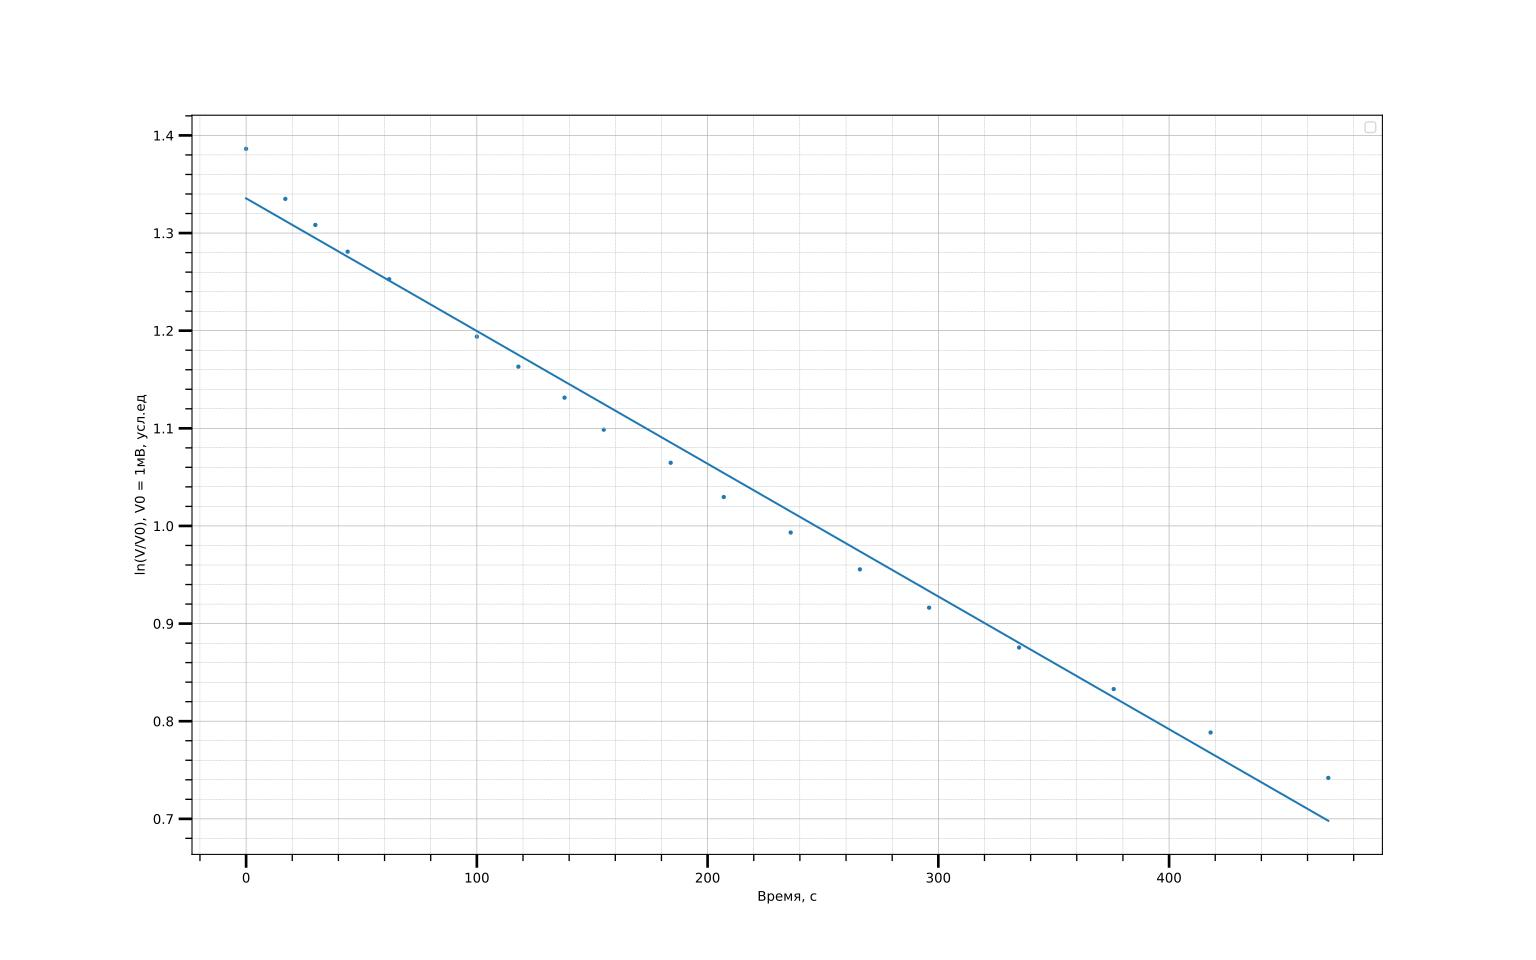
\includegraphics[width=16cm]{graphik22.jpg}
    \caption{График зависимости логарифма напряжения от времени при рабочем давлении Р = 22 торр}
    \label{fig:}
  \end{center}
\end{figure}

\begin{figure}[H]
  \begin{center}
    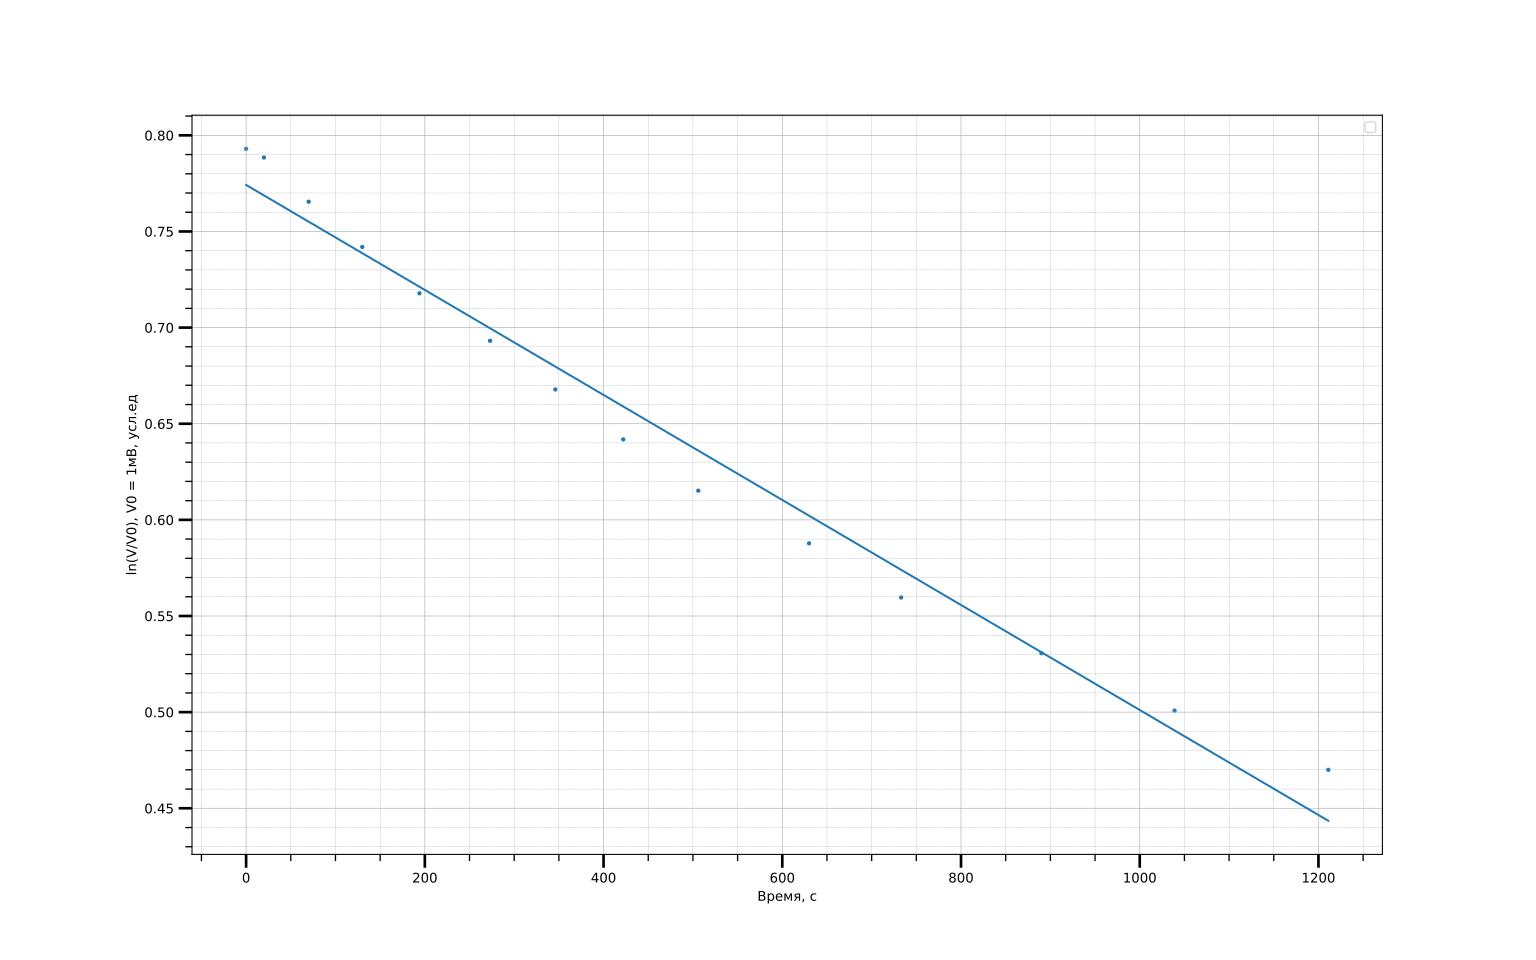
\includegraphics[width=16cm]{graphik33.jpg}
    \caption{График зависимости логарифма напряжения от времени при рабочем давлении Р = 33 торр}
    \label{fig:}
  \end{center}
\end{figure}

\begin{figure}[H]
  \begin{center}
    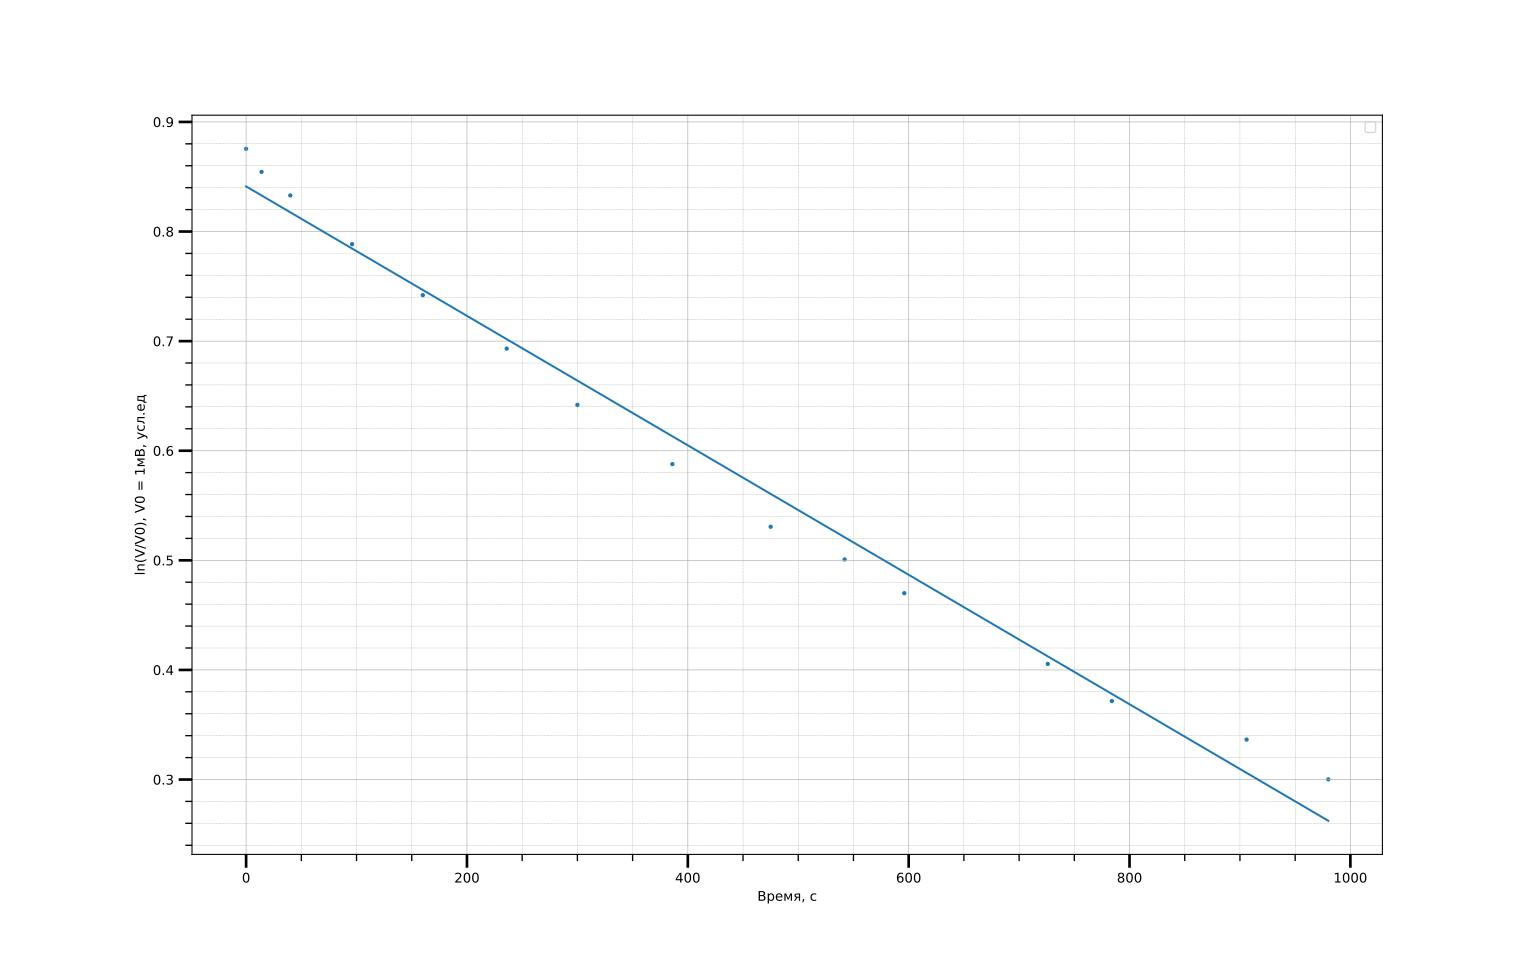
\includegraphics[width=16cm]{graphik45.jpg}
    \caption{График зависимости логарифма напряжения от времени при рабочем давлении Р = 45 торр}
    \label{fig:}
  \end{center}
\end{figure}

\begin{figure}[H]
  \begin{center}
    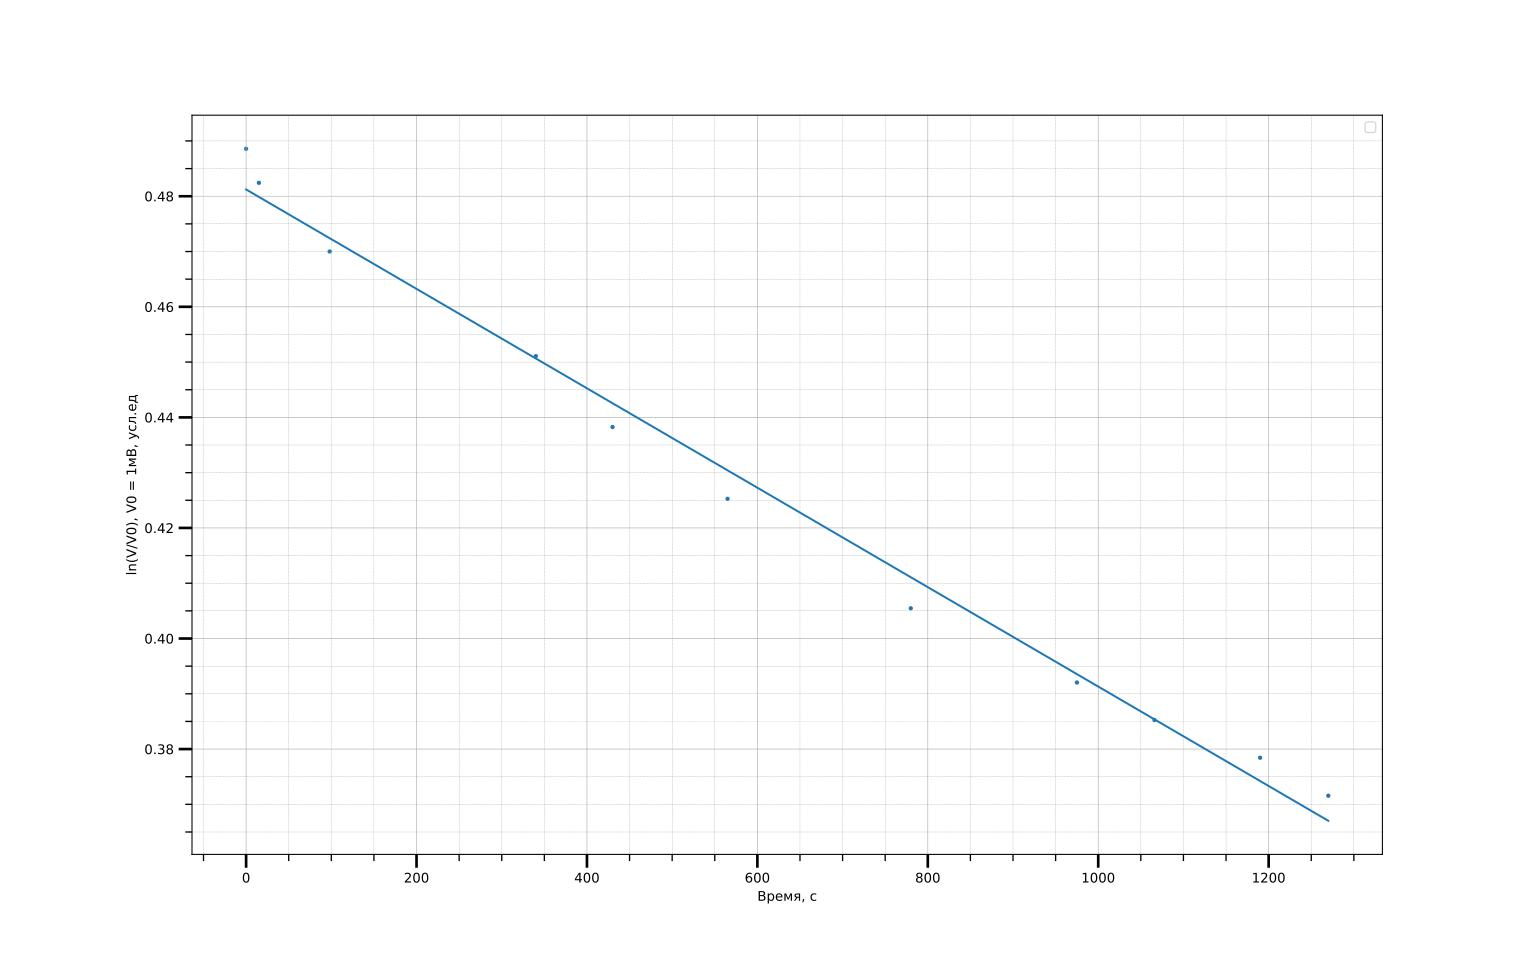
\includegraphics[width=16cm]{graphik55.jpg}
    \caption{График зависимости логарифма напряжения от времени при рабочем давлении Р = 55 торр}
    \label{fig:}
  \end{center}
\end{figure}

Графики имеют вид прямых линий, значит зависимость действительно экспоненциальная. Теперь по наклонам экспериментальных прямых и по известным параметрам установки рассчитываем коэффициенты диффузии через пористое тело. Обозначим за k угловой коэффициент наклона графика, тогда
\[ \frac{1}{k} = -\frac{V_1 V_2 L}{S D_p (V_1 + V_2)} \]
значит 
\[D_p = -\frac{V_1 V_2 L k}{S  (V_1 + V_2)}  \]
обозначим $\gamma = -\frac{V_1 V_2 L}{S (V_1 + V_2)} $, тогда $D_p = \gamma k$

$\gamma = 0.017\pm 0.003 м^{2}$
\[ \sigma_{\gamma } = \gamma \sqrt{2\left(\frac{\sigma_{V}}{(V)}\right)^2+\left(\frac{\sigma_{2V}}{(2V)}\right)^2+\left(\frac{\sigma_{S}}{(S)}\right)^2+\left(\frac{\sigma_{L}}{(L)}\right)^2} \]

Угловые коэффициенты и их случайную ошибку определяем по формулам


\begin{equation}\label{mnk:k}
k=\frac{\langle t\ln V/V_0 \rangle - \langle t\rangle \langle \ln V/V_0\rangle}{\langle t^2 \rangle - \langle t \rangle^2}
\end{equation}

\[ \sigma^\text{случ}_k = \sqrt{\frac{1}{N}\frac{\langle ln(V/V_0)^{2}\rangle - \langle ln(V/V_0)\rangle^{2}}{\langle t^{2}\rangle - \langle t\rangle^{2}}- k^{2}} \]


где N -- колличество измерений. При этом можно считать, что $ \sigma_k \approx \sigma_k^\text{случ} $, т.к. показания вольтметра довольно точны и систематическая ошибка мала по сравнению со случайными флуктуациями напряжения в ходе эксперимента.

Погрешность коэффициента взаимной диффузии можно вычислить по следующей формуле:
\[ \sigma_D = D\sqrt{\left(\frac{\sigma_k}{k}\right)^2+\left(\frac{\sigma_{\gamma }}{(\gamma )}\right)^2} \]

Проводя данные вычисления для каждого значения, заносим результаты в таблицу.

\begin{table}[H]
	\centering
	\begin{tabular}{|c|c|c|c|c|c|}
		\hline
		$ P $, торр & $ \sigma_P $, торр & $ k \cdot 10^{-3} $, с$ ^{-1} $ & $ \sigma_{k} \cdot 10^{-3} $, с$ ^{-1} $ & $ D $, $ cm^{2}/c $ & $ \sigma_D $, $ cm^{2}/c $ \\ \hline
		22 & 1 & -1.359 & 0.038 & 0.230 & 0.040 \\ \hline
		33 & 1 &  -0.591&  0.018& 0.100 & 0.015 \\ \hline
		45 & 1 & -0.273 & 0.010 & 0.045 & 0.007 \\ \hline
		55 & 1 & -0.0899 & 0.0027 & 0.015 & 0.002 \\ \hline
	
	\end{tabular}
	\caption{Аппроксимация зависимостей}
	\label{tab:approx}
\end{table}

Строим график зависимости обратного коэффициента диффузии от давления. По нему видно, что при увеличении величины, обратной давлению, коэффициент диффузии возрастает. Из данного графика нельзя сделать вывод о прямой пропорциональности, как предсказывает теория.

\begin{figure}[H]
  \begin{center}
    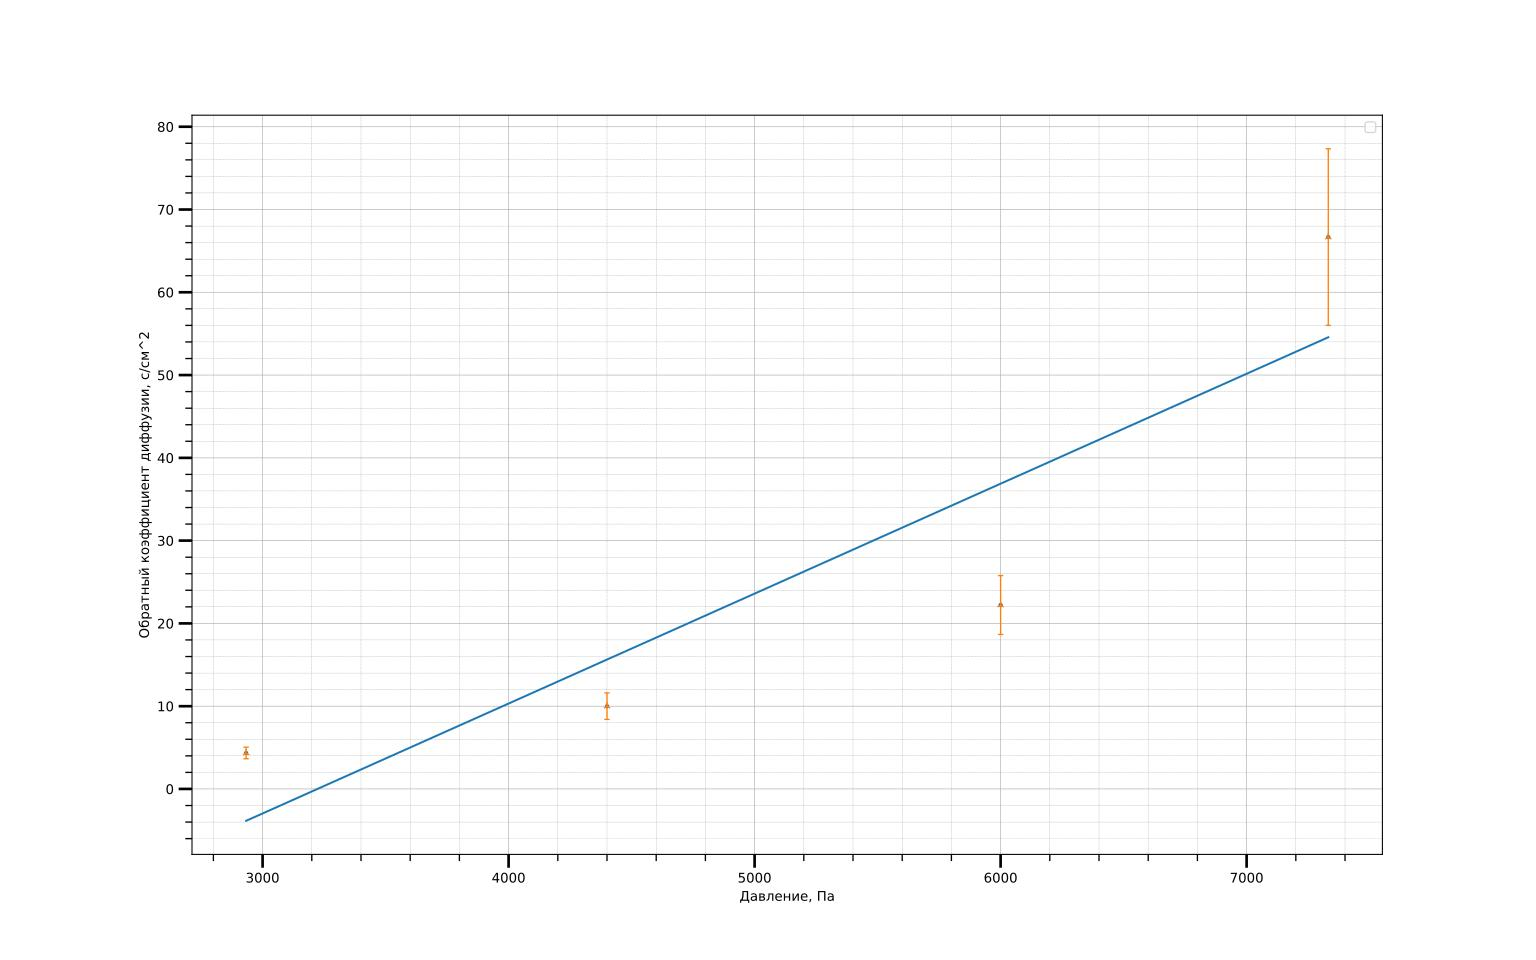
\includegraphics[width=16cm]{graphikD.jpg}
    \caption{График зависимости обратного коэффициента диффузии от давления}
    \label{fig:}
  \end{center}
\end{figure}

Определим коэффициент пористости среды $ \delta \xi^{2} $, зная, что коэффициент диффузии гелия в открытом пространстве при давлении 760 торр равен $ D = 0.3  cm^{2}/c$.


Значит, D пропорционален 1/P с коэффициентом $ m = D/(1/P) = DP = 3.04 m^{2}$ * Па/с.
Значит
\[ \frac{1}{D_p}  = \frac{1}{\delta \xi^{2} D} + \frac{1}{D_{K_{p}}} =\frac{P}{\delta \xi^{2} m} + \frac{1}{D_{K_{p}}}  \]
и угловой коэффициент  $\rho$ наклона графика зависимости обратного коэффициента диффузии от давления равен 
\[ \rho = \frac{1}{\delta \xi^{2} m} \Rightarrow \delta \xi^{2} = \frac{1}{m\rho} \]



Тем же методом, что и коэффициенты в предыдущих графиках, определяем $\rho $ = 132789 $\pm $ 32396 $\frac{c}{m^{2}*Pa}$, значит коэффициент пористости $ \delta \xi^{2} = 0.025\pm 0.006 $ Если считать $\xi \approx \delta $, то этот результат означает, что обЪем, занятый порами, занимает примерно треть обЪема всей пористой среды.

Найдем коэффициент диффузии при малых давлениях
\[ D_{K_p} = \frac{1}{\frac{1}{D_p}+\frac{1}{D\delta \xi^{2}}} = (2.6\pm  0.7 )* 10^{-9} m^{2}/c\]
значит кнудсеновский коэффициент диффузии равен
\[ D_K = \frac{D_{K_p}}{\delta \xi^{2}} = (1.0\pm 0.3) * 10^{-7} m^{2}/c\]

учитывая, что
\[ D_K = \frac{d}{3} \sqrt{\frac{8RT}{\pi \mu }}\]
при Т = 300К
\[ d = 3D_K\sqrt{\frac{\pi \mu }{8RT}} = (1.7\pm 0.4) * 10^{-10} m \]

Кнудсеновская диффузия — диффузия газа через сквозные поры в твёрдых телах, непроницаемых для газов при относительно малых давлениях газа или размерах пор, то есть в случаях, когда длина свободного пробега $\lambda $ молекул много больше характерного диаметра пор d. Переход от обычной диффузии в газах в кнудсеновскую характеризуют безразмерным параметром — числом, или критерием Кнудсена — Kn
\[ K_n = \frac{\lambda }{d} \approx 10^{-3}\Rightarrow \lambda = K_n  d\]
учитывая, что 
\[ \lambda = \frac{k_b  T}{4\sqrt{2}\pi d^{2} P}\Rightarrow P = \frac{k_b  T}{4\sqrt{2}\pi d^{2} \lambda } = \frac{k_b  T}{4\sqrt{2}\pi d^{2} K_n d} = 10^{11} Pa\]

\section{Обсуждение результатов и выводы}

В данной лабораторной работе была исследована зависимость концентрации гелия в воздухе от времени при различных начальных давлениях смеси. Было выяснено, что при увеличении давления, коэффициент диффузии уменьшается, это связано с увеличением количества столкновений между молекулами. 

Также был определен коэффициент диффузии гелия в пористой среде, его значение при давлении 22 торр составило $0.23\pm 0.4 cm^2/c $, это меньше коэффициента диффузии в открытой среде $\sim $ 10 $cm^2/c$. 

Были вычислены геометрические характеристики пористой среды, такие как отношение объема, занятого порами, к объему всего пористого тела, значение которого составило примерно 0.3, и средний диаметр пор, который составил примерно 0.2 нм. 

Диффузия в данной работе проходила в кнудсеновском режиме, для перехода к вязкостному при том же диаметре пор необходимо поднять давление до 1 млрд торр.


\end{document}
	
